\section*{Results}

\begin{table}[htp]
  \centering
  \csvautotabular{../processed_data/algorithm_time.csv}
  \caption{Average (20 runs) algorithm run times in seconds.}
  \label{table:summary}
\end{table}


From the summary (\cref{table:summary}) we immediately see that the
TDCMA is slower than TDMA and the LU is considerably slower than both TDMA and
TDCMA.



To see how the algorithm time for our different methods scales with N we divide
all timings with N (\cref{table:normalized}). Both TDMA and TDCMA run times are
of the same order, as was expected from the counting of flops. The times for LU
show an increase of two orders of magnitude for each magnitude increase in n.
This is consistent with our expectations of the LU algorithm time being
proportional to $n^3$.

\begin{table}[htp]
  \centering
  \csvautotabular{../processed_data/normalized.csv}
  \caption{Algorithm times divided by n.}
  \label{table:normalized}
\end{table}


Comparing the run times of TDMA and TDCMA (\cref{table:comparison})
we see they are the same order of magnitude. Theoretically we would
expect TDCMA to be $\frac{9 FLOPS}{4 FLOPS} \approx 2.25$ times as fast as
TDMA. When counting FLOPS we did not consider memory operations, so getting as
these values close to 2.25 is considered to be in agreement with the theory.

\begin{table}[htp]
  \centering
  \csvautotabular{../processed_data/comparison.csv}
  \caption{Run times of algorithms compared to TDCMA.}
  \label{table:comparison}
\end{table}


\Cref{fig:a} shows that we get quite good agreement with the analytic solution
when N goes to 1000. To investigate further we look at the relative error
$\epsilon_i = \abs{\frac{u_i - v_i}{u_i}}$ in \cref{fig:a}.
When increasing N (decreasing the step size h) up to $10^6$ the relative error
decreases proportionally, until N = $10^7$, which might be a sign that we are
starting to experience some round off errors.


\begin{figure}[htp]
  \centering
  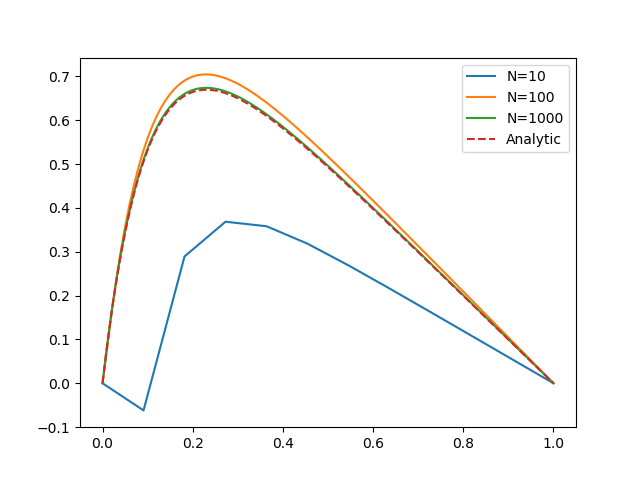
\includegraphics[width=0.66\textwidth]{../figures/TDMA.png}
  \caption{Comparison of analytic solution and numerical approximations with TDMA.}
  \label{fig:a}
\end{figure}


\begin{figure}[htp]
  \centering
  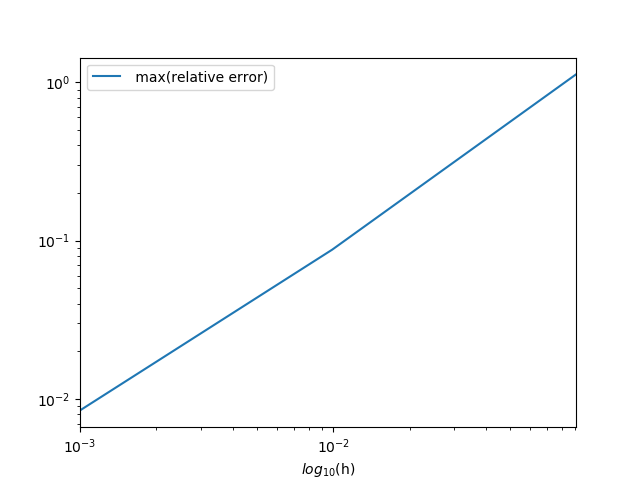
\includegraphics[width=0.66\textwidth]{../figures/relative_error.png}
  \caption{Maxmimum relative error between analytical and TDMA solution.}
  \label{fig:relative_error}
\end{figure}
